\documentclass[conference]{IEEEtran}
\IEEEoverridecommandlockouts
\usepackage{cite}
\usepackage{amsmath,amssymb,amsfonts,bm}
\usepackage{graphicx}
\usepackage{textcomp}
\usepackage{xcolor}
\usepackage[ruled,vlined,linesnumbered]{algorithm2e}
\usepackage{booktabs,multirow,array,tabularx,longtable,colortbl}
\usepackage{tikz}
\usetikzlibrary{arrows.meta,positioning,fit,backgrounds,calc,shapes.geometric,patterns,decorations.pathreplacing}
\usepackage{amsthm}
\newtheorem{assumption}{Assumption}
\newtheorem{lemma}{Lemma}
\newtheorem{theorem}{Theorem}
\newtheorem{corollary}{Corollary}
\newtheorem{proposition}{Proposition}
\renewcommand{\theassumption}{S\arabic{assumption}}
\renewcommand{\thelemma}{S\arabic{lemma}}
\renewcommand{\thetheorem}{S\arabic{theorem}}
\renewcommand{\thecorollary}{S\arabic{corollary}}
\renewcommand{\theproposition}{S\arabic{proposition}}
\theoremstyle{remark}
\newtheorem{remark}{Remark}
\renewcommand{\theremark}{S\arabic{remark}}
\usepackage{hyperref}
\hypersetup{colorlinks=true,linkcolor=blue,citecolor=blue,urlcolor=blue,filecolor=blue}
\newcommand{\Eqref}[1]{\textcolor{blue}{(\ref{#1})}}
\definecolor{bestblue}{RGB}{214,232,245}
\newcommand{\cP}{\mathcal{P}}
\newcommand{\cN}{\mathcal{N}}
\newcommand{\cA}{\mathcal{A}}
\newcommand{\cE}{\mathcal{E}}
\newcommand{\cO}{\mathcal{O}}
\newcommand{\cU}{\mathcal{U}}
\newcommand{\cD}{\mathcal{D}}
\newcommand{\cR}{\mathcal{R}}
\newcommand{\cF}{\mathcal{F}}
\newcommand{\cJ}{\mathcal{J}}
\newcommand{\cM}{\mathcal{M}}
\newcommand{\cV}{\mathcal{V}}
\newcommand{\cC}{\mathcal{C}}
\newcommand{\cL}{\mathcal{L}}
\newcommand{\cB}{\mathcal{B}}
\newcommand{\cG}{\mathcal{G}}
\newcommand{\cI}{\mathcal{I}}
\newcommand{\cH}{\mathcal{H}}
\newcommand{\cX}{\mathcal{X}}
\newcommand{\cS}{\mathcal{S}}
\renewcommand{\theequation}{S\arabic{equation}}
\renewcommand{\thetable}{S\arabic{table}}
\renewcommand{\thefigure}{S\arabic{figure}}
\renewcommand{\thealgocf}{S\arabic{algocf}}
\setlength{\abovedisplayskip}{4pt plus 1pt minus 1pt}
\setlength{\belowdisplayskip}{4pt plus 1pt minus 1pt}
\setlength{\textfloatsep}{7pt plus 2pt minus 2pt}
\setlength{\dbltextfloatsep}{7pt plus 2pt minus 2pt}
\renewcommand{\topfraction}{0.93}
\renewcommand{\dbltopfraction}{0.93}
\renewcommand{\textfraction}{0.07}
\begin{document}

\title{\fontsize{16}{19}\selectfont Supplementary Material for A Critical-Path Guided Multi-agent Reinforcement Learning framework based on Heterogeneous Graph Attention with Critical-Slack Action Ranking and Precedence-Certified Decoding for Reliability-Aware Dynamic Flexible Job Shop Scheduling under Machine Breakdowns}

\author{%
\begin{tabular}{@{}c@{\hspace{0.06\textwidth}}c@{}}
\begin{minipage}[t]{0.44\textwidth}\centering
{\sublargesize \mbox{1st Xian Li}}\\[0.35em]
{\normalsize School of Information Engineering and Automation\\
Kunming University of Science and Technology\\
Kunming, China\\
20242204247@stu.kust.edu.cn}
\end{minipage}
&
\begin{minipage}[t]{0.44\textwidth}\centering
{\sublargesize \mbox{2nd Zi-Qi Zhang\textsuperscript{*}}}\\[0.35em]
{\normalsize School of Information Engineering and Automation\\
Kunming University of Science and Technology\\
Kunming, China\\
zhangziqi@kust.edu.cn}
\end{minipage}\\[0pt]
\begin{minipage}[t]{0.44\textwidth}\centering
\vspace*{0.7em}%
{\sublargesize \mbox{3rd Xiao-Ting~An$^{*}$}}\\[0.35em]
{\normalsize Academic Affairs Office of YJPU\\
Yunnan Jiaotong Polytechnic University\\
Kunming, China\\
2019082252@ynjtc.edu.cn}
\end{minipage}
&
\begin{minipage}[t]{0.44\textwidth}\centering
\vspace*{0.7em}%
{\sublargesize \mbox{4th Bin Qian}}\\[0.35em]
{\normalsize School of Information Engineering and Automation\\
Kunming University of Science and Technology\\
Kunming, China\\
bin.qian@kust.edu.cn}
\end{minipage}
\end{tabular}}

\maketitle

\begin{abstract}
This supplement documents the complete formulation, implementation, convergence analysis, and experimental statistics of CPR-PPO, including TRAE, CSAR, PCD, CPR-S, and KACP. Section~I fixes the notation and the event mechanics. Section~II details the heterogeneous graph and the typed attention encoder. Section~III states the decision process, the decoder, and the release properties, Section~IV documents training, and Section~V proves convergence. Section~VI derives the time and memory complexity, Section~VII reports the per-unit and paired statistics, and Section~VIII states the reproducibility protocol. Equation, table, figure, and algorithm numbers carry the prefix S and are distinct from those of the manuscript.
\end{abstract}

\begin{IEEEkeywords}
Supplementary material, dynamic flexible job-shop scheduling, machine breakdowns, heterogeneous graph attention, multi-agent reinforcement learning, proximal policy optimization.
\end{IEEEkeywords}

\section{Notation and Event Mechanics}
\label{sec:S-notation}

\subsection{Symbol Table}
\label{sec:S-symbols}

Table~\ref{tab:S-symbols} lists every symbol used in the manuscript and in this supplement. Sets use calligraphic capitals, vectors and matrices bold italic, scalars italic, and operators upright; $|\cdot|$ is cardinality and $[\bm{x};\bm{y}]$ concatenation.

\begin{table*}[!t]
\caption{Symbols and meanings.}
\label{tab:S-symbols}
\centering
\scriptsize
\setlength{\tabcolsep}{3pt}
\begin{tabular}{@{}p{1.75cm}p{6.05cm}p{1.75cm}p{6.05cm}@{}}
\toprule
\textbf{Symbol} & \textbf{Meaning} & \textbf{Symbol} & \textbf{Meaning}\\
\midrule
$\cJ,\cM,\cO$ & sets of jobs, machines and operations & $n,m$ & number of jobs and machines\\
$\cM_o$ & eligible machine set of operation $o$ & $\cP(o)$ & immediate job and machine predecessors\\
$\cN^{+}(o)$ & immediate job and machine successors & $\cC(o)$ & descendants of $o$ in the decoded graph\\
$\cD_\tau,\cR_\tau,\cU_\tau$ & completed, running, unstarted or interrupted operations & $\cF_\tau$ & frozen set, $\cD_\tau\cup\cR_\tau$\\
$p_{o,k}$ & processing time of $o$ on machine $k$ & $p_{\mathrm{ref}}$ & median eligible processing time\\
$q$ & failure probability of an attempt of length $p_{\mathrm{ref}}$ & $\lambda$ & constant failure rate\\
$r_{\min},r_{\max}$ & repair duration bounds & $R_k$ & known repair completion of machine $k$\\
$\tau_j$ & instant of the $j$-th breakdown & $k_o$ & machine assigned to $o$\\
$s_o,c_o$ & start and completion times of $o$ & $a_o$ & release bound of $o$\\
$\Delta_o$ & reservation duration, $c_o-s_o$ & $\sigma_o$ & critical slack of $o$\\
$LS_o$ & latest start time of $o$ & $\hat{C}_{\max}(S)$ & nominal makespan of schedule $S$\\
$C_i^{\mathrm{act}}$ & realized completion time of job $i$ & $C_{\mathrm{ref}}$ & initial nominal makespan, lower-clipped at one\\
$\gamma$ & discount factor ($\gamma=1$) & $\cG=(\cV,\cE,\bm{H})$ & heterogeneous graph\\
$\cV=\cO\cup\cM$ & node set & $\cE$ & typed edge set\\
$\bm{e}_{uv}$ & edge features, $\mathbb{R}^3$ & $\bm{h}_u$ & node embedding\\
$\bm{W}_{Q,K,V}$ & attention projections & $\bm{w}_e$ & edge weight\\
$\alpha_{uv}$ & attention weight & $\bm{m}_u$ & aggregated message\\
$d,H,L,d_h$ & width (48), heads (4), layers (2), head width (12) & $d_O,d_M,d_E$ & operation (12), machine (9), edge (3) features\\
$d_A,d_G$ & candidate (6) and global (5) features & $\bm{x}_a$ & candidate feature vector\\
$\bm{g}$ & pooled context, $\mathbb{R}^{2d+5}$ & $z_a$ & action logit\\
$\pi_\theta,V_\phi$ & actor and critic & $\cA(s)$ & joint relocation set\\
$S_L,S_E,S_{\mathrm{out}}$ & learning, search and released schedules & $\varepsilon_{\mathrm{tol}}$ & nominal improvement threshold\\
$L_s,B_L,B_G$ & search memory (5), learning and search budgets (96) & $r_j,t_j$ & reward and production time of decision $j$\\
$\cD$ & demonstration set of pairs $(s,a^{*})$ & $\beta,\delta$ & ranking weight and logit margin\\
$\rho_j,\hat{A}_j$ & probability ratio and advantage estimate & $\epsilon$ & clipping range\\
$c_v,c_e,c_k$ & value, entropy and KL weights & $\pi_{\mathrm{clone}}$ & frozen cloned policy\\
$\eta,\nu$ & unit and instance indices & $C_{\nu b},C^{*}_{\nu}$ & realized makespan and empirical reference\\
$G_{\eta b},G_b$ & unit and mean empirical gap & $R_{\eta b},R_b$ & unit and mean rank\\
\bottomrule
\end{tabular}
\end{table*}

\subsection{Event Handler}
\label{sec:S-events}

Algorithm~\ref{alg:S-event} states the event handler invoked at every breakdown. At $\tau_j$, completed and running operations are frozen, an interrupted operation moves to $\cU_\tau$ with release bound $R_{k^\dagger}$, and online arrivals are appended to $\cU_\tau$. A relocation that crosses a frozen reservation is blocked. The policy observes only the graph snapshot, future failures remain hidden, and the next breakdown ends the epoch. The handler therefore defines the transition from the physical shop state to the decision state, and it returns the quantities consumed by the two recovery branches.

\begin{algorithm}[!t]
\caption{Event handling and state transition at a breakdown}
\label{alg:S-event}
\footnotesize
\SetKwInOut{Input}{Input}
\SetKwInOut{Output}{Output}
\Input{shop state $\cX$, instant $\tau$, failed machine $k^{\dagger}$, repair sampler}
\Output{frozen set $\cF_\tau$, movable set $\cU_\tau$, repair completions $\{R_k\}$, graph $\cG$}
$R_{k^{\dagger}}\leftarrow \tau+\mathrm{Repair}(k^{\dagger})$\;
\ForEach{$o\in\cO$}{
  \uIf{operation $o$ completed before $\tau_j$}{add $o$ to $\cD_\tau$}
  \uElseIf{$o$ is running at $\tau_j$ on $k\ne k^{\dagger}$}{add $o$ to $\cR_\tau$; keep recorded $(k_o,s_o,c_o)$}
  \uElseIf{$o$ is running at $\tau_j$ on $k^{\dagger}$}{add $o$ to $\cU_\tau$; keep $k_o=k^{\dagger}$; set release bound $a_o=R_{k^{\dagger}}$; discard partial progress}
  \Else{add $o$ to $\cU_\tau$}
}
append online arrivals to $\cU_\tau$; set $a_o=\tau$ for each new arrival\;
$\cF_\tau\leftarrow\cD_\tau\cup\cR_\tau$; freeze $(k_o,s_o,c_o)$ for $o\in\cF_\tau$\;
compute $R_k$ for every machine under repair, and $R_k\leftarrow\tau$ otherwise\;
build $\cG$ from $(\cF_\tau,\cU_\tau,\{R_k\})$ with the incidence rule of Section~II\;
\Return{$\cF_\tau,\cU_\tau,\{R_k\},\cG$}
\end{algorithm}

\section{Mathematical Model}
\label{sec:S-model}

Fig.~\ref{fig:S-shop} illustrates the physical context of DFJSP-MB. Shop-level planning releases jobs, selects routes, and allocates operations to machines; cell-level execution runs the machines, AGV material flow, buffers, and the repair crew. A breakdown at $\tau$ isolates the failed machine $k^{\dagger}$ over the repair interval $[\tau_j,R_k]$, and the interrupted operation loses its progress and restarts on $k^{\dagger}$ after repair. Completed and running operations form the frozen set $F_\tau=D_\tau\cup R_\tau$, whereas unstarted operations and interrupted operations form $U_\tau$; the latter restart on the same machine under the release bound $a_o=R_k$. The figure is contextual; the formal event transition is given in Section~I-B.

\begin{figure*}[!t]
\centering
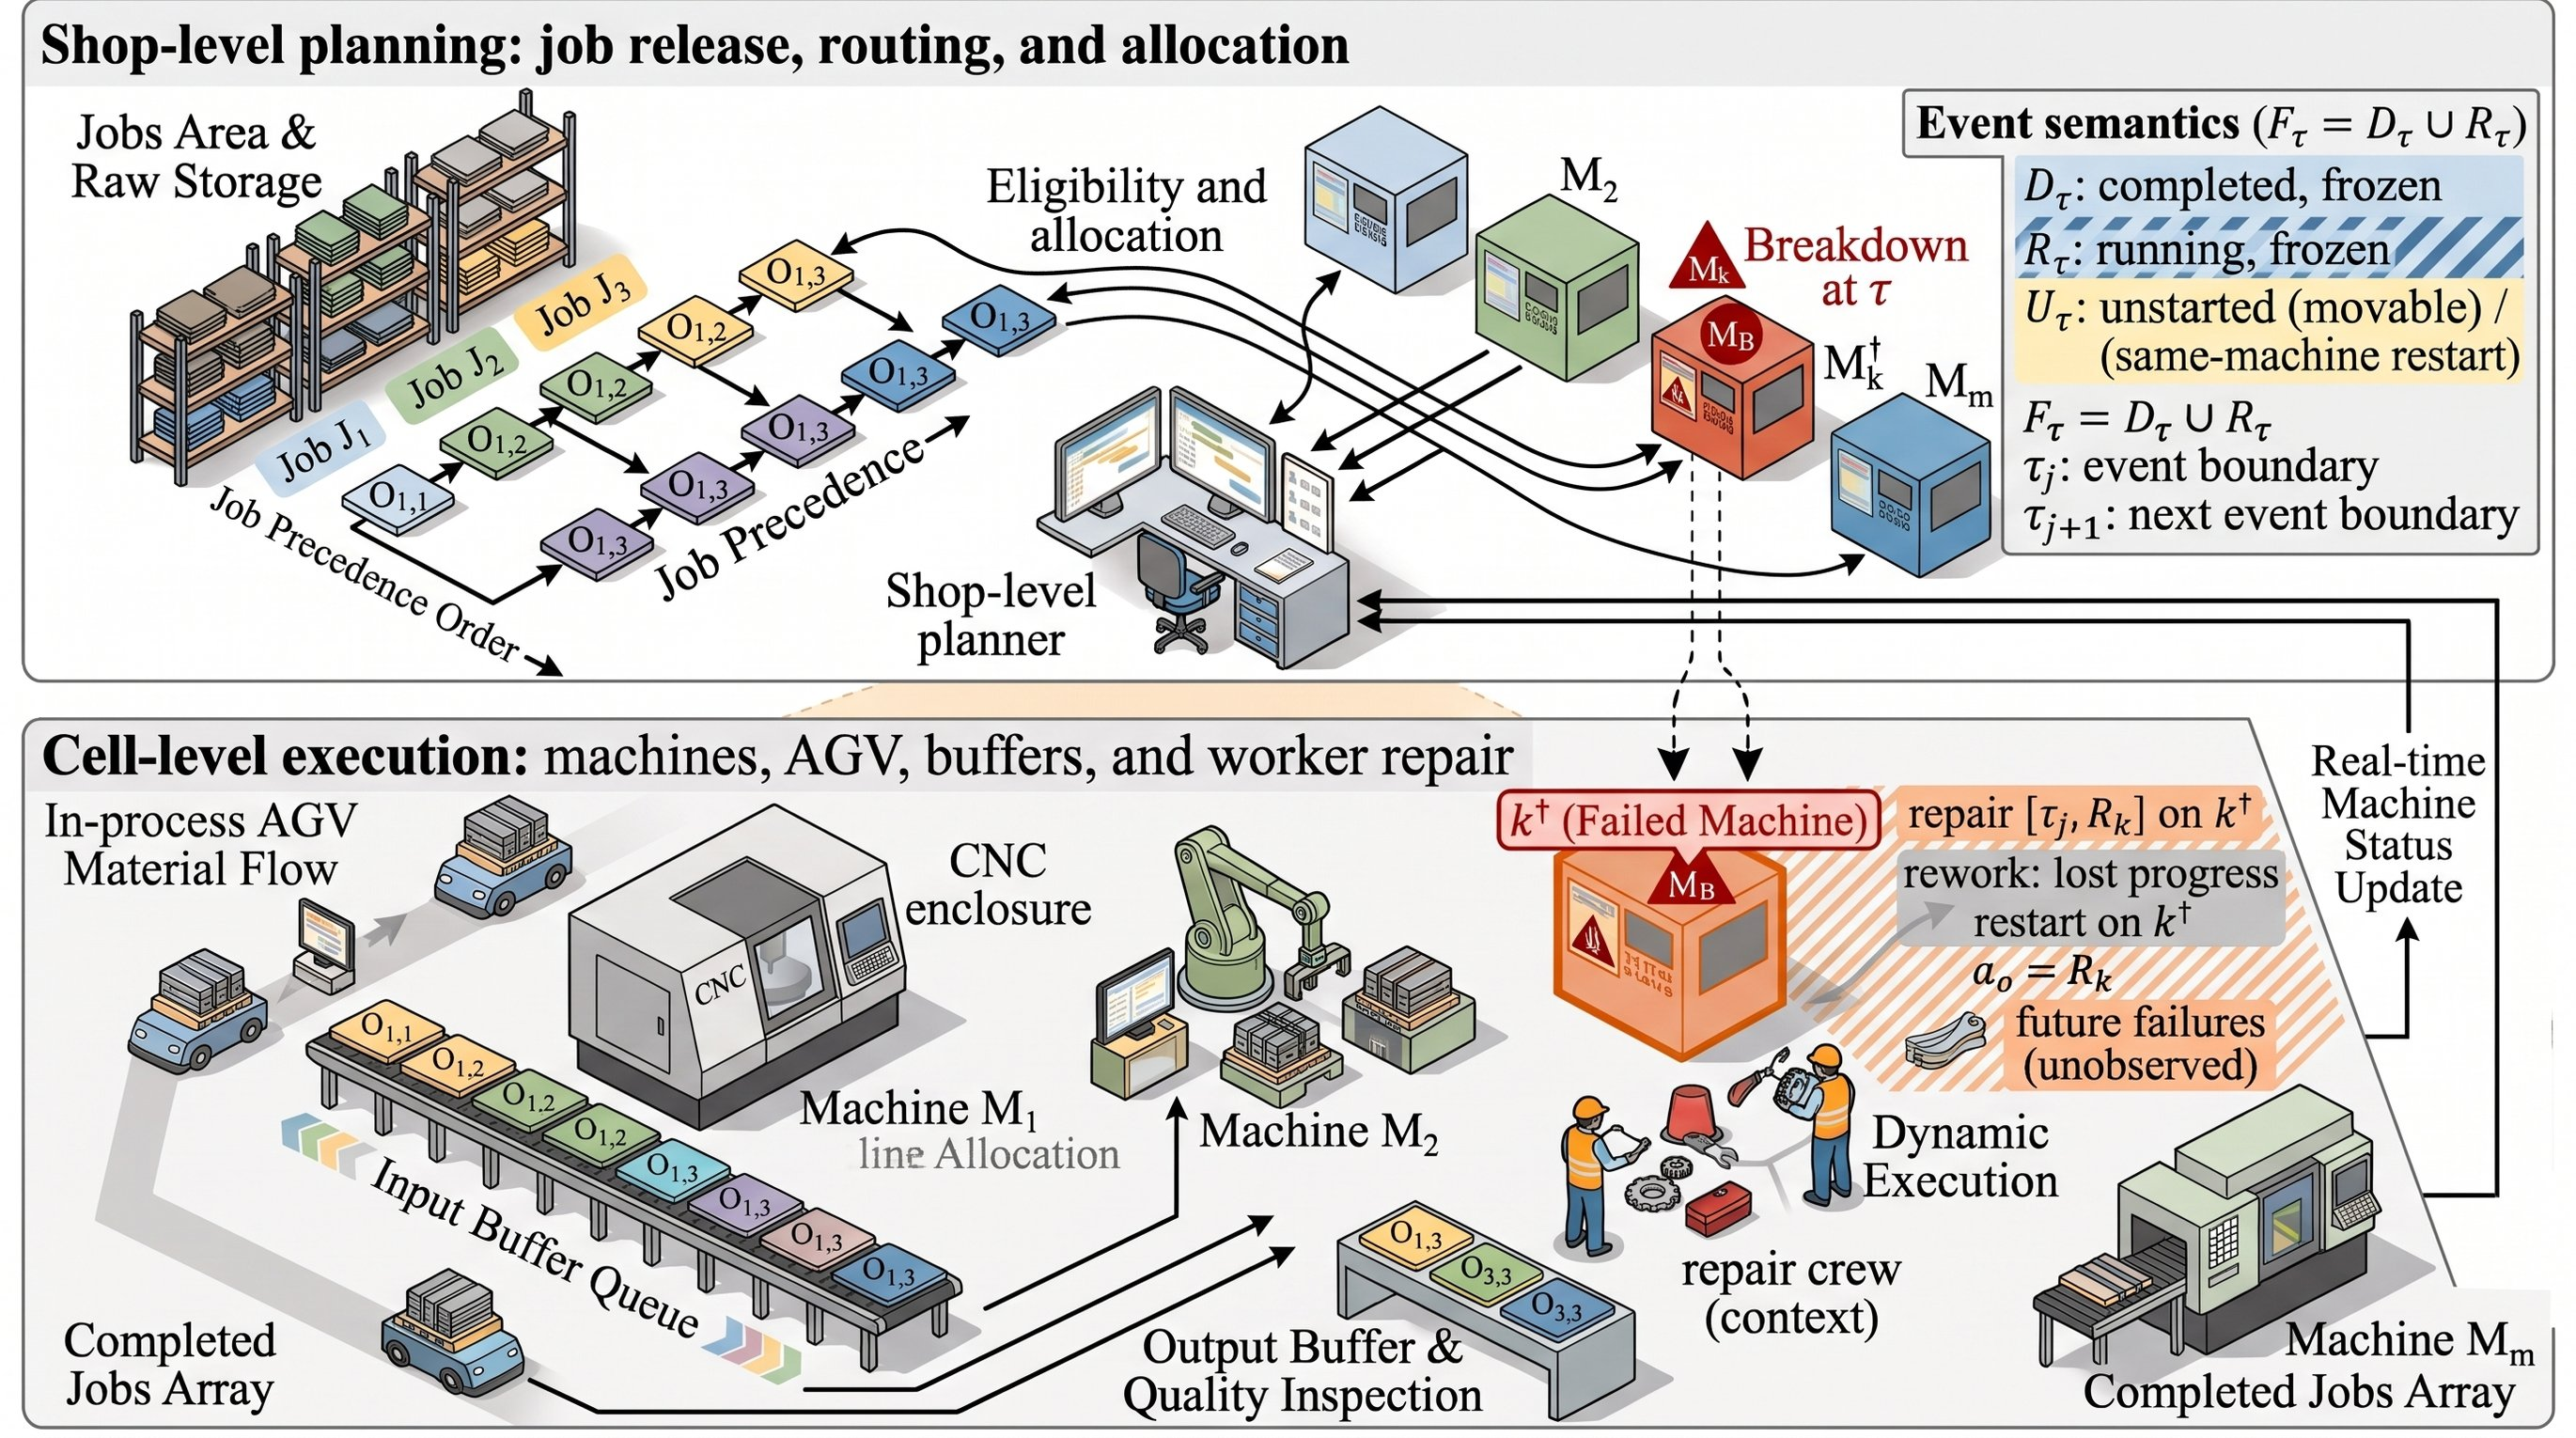
\includegraphics[width=0.73\textwidth]{figs/figS_shop.jpg}
\caption{Shop context of DFJSP-MB. Frozen $D_\tau\cup R_\tau$ keep their reservations and only $U_\tau$ is movable; $a_o=R_k$ is the restart bound.}
\label{fig:S-shop}
\end{figure*}

\subsection{Feasibility Constraints}
\label{sec:S-feasibility}

For a recovery schedule $S$, let $k_o$, $s_o$, and $c_o$ denote the assigned machine, start time, and completion time of operation $o$. The duration identity is
\begin{equation}
c_o=s_o+p_{o,k_o},\qquad o\in\cU_\tau,
\label{eq:S-duration}
\end{equation}
and the assignment satisfies
\begin{equation}
k_o\in\cM_o,\qquad o\in\cU_\tau.
\label{eq:S-elig}
\end{equation}
A schedule is feasible if
\begin{equation}
\left\{
\begin{aligned}
&\underbrace{k_o\in\cM_o,\quad c_o=s_o+p_{o,k_o}}_{\text{eligibility and duration}},\quad o\in\cU_\tau,\\
&\underbrace{c_v\le s_o}_{\text{job precedence}},\quad v\in\cP_J(o),\\
&\underbrace{c_o\le s_v\ \text{or}\ c_v\le s_o}_{\text{machine non-overlap}},\quad k_o=k_v,\ o\ne v,\\
&\underbrace{s_{o^{\dagger}}\ge R_{k^{\dagger}}}_{\text{restart bound}},\quad
\underbrace{(k_o,s_o,c_o)\ \text{fixed}}_{\text{frozen reservation}},\quad o\in\cF_\tau,
\end{aligned}
\right.
\label{eq:S-feas}
\end{equation}
where $\cP_J(o)$ is the immediate job predecessor and $o^{\dagger}$ is an interrupted operation. The first line states eligibility and duration, the second states job precedence, the third states machine non-overlap, and the fourth states the restart bound and frozen reservations. For fixed queues, these arcs form a directed acyclic graph.

\subsection{Markov Decision Process}
\label{sec:S-mdp}

The decision process is the tuple $(\cS,\cA,T,r,\Omega,\gamma)$. A decision state is
\begin{equation}
s=(\cG,\cF_\tau,\cU_\tau,\{R_k\},B),
\label{eq:S-state}
\end{equation}
where $\cG$ is the heterogeneous graph, $B$ is the remaining candidate budget, and the other symbols follow Section~I. The action space is
\begin{equation}
\cA(s)=\bigcup_{k\in\cM}\cA_k(s),
\label{eq:S-action}
\end{equation}
where a relocation is
\begin{equation}
a=(o,k,h)\in\cA(s),
\label{eq:S-reloc}
\end{equation}
where $\cA_k(s)$ contains relocations proposed by the agent of machine $k$. The transition $s'=T(s,a,\xi)$ applies the decoder of Section~IV-B to an accepted move and leaves $s$ unchanged for a rejected move. The reward is
\begin{equation}
r_j=-\frac{t_{j+1}-t_j}{C_{\mathrm{ref}}},
\label{eq:S-reward}
\end{equation}
with discount
\begin{equation}
\gamma=1,
\label{eq:S-gamma}
\end{equation}
so the return telescopes to the negative normalized realized production time. The observation $\Omega(s)=\cG$ masks health and risk channels; the hidden component is the future failure stream. Table~\ref{tab:S-state} lists the state features and Table~\ref{tab:S-action} lists the action attributes.

\section{TRAE: Heterogeneous Graph and Attention}
\label{sec:S-graph}

\subsection{Graph Construction}
\label{sec:S-construction}

The graph has operation and machine nodes, $\cV=\cO\cup\cM$. Job-precedence arcs connect consecutive operations of a job and carry the type \emph{precedence}; compatibility edges connect an operation to each machine in its eligible set and carry the type \emph{eligibility}. For an edge $uv$, the feature vector $\bm{e}_{uv}\in\mathbb{R}^{3}$ stores the processing time, a binary original-assignment flag, and a type indicator. Operation features follow Table~S2; machine features encode repair completion, reserved load, queue length, and availability. The construction is $O(|\cO|+|\cE|)$ in time and memory.

\begin{table}[!t]
\caption{Observation features. Every feature is normalized to $[-1,1]$ by fixed constants.}
\label{tab:S-state}
\centering
\scriptsize
\setlength{\tabcolsep}{3pt}
\begin{tabular}{@{}p{1.15cm}p{0.45cm}p{5.0cm}@{}}
\toprule
\textbf{Group} & \textbf{Dim} & \textbf{Feature}\\
\midrule
Operation & 12 & remaining job work; processing time; mean eligible time; earliest start; recorded start and completion; slack; status; eligibility count; job position; successor and predecessor counts\\
Machine & 9 & repair completion $R_k$; repair flag; reserved load; queue length; mean queued time; earliest availability; frozen queued count; utilization; free capacity\\
Edge & 3 & processing time; original-assignment flag; type indicator\\
Candidate & 6 & critical slack; completion change; blocking; chain length; eligibility count; insertion depth\\
Global & 5 & frozen fraction; repair fraction; mean queue length; remaining-work ratio; nominal makespan\\
\bottomrule
\end{tabular}
\end{table}

\begin{table}[!t]
\caption{Action space, candidate attributes, and rejection rule.}
\label{tab:S-action}
\centering
\scriptsize
\setlength{\tabcolsep}{3pt}
\begin{tabular}{@{}p{1.55cm}p{5.55cm}@{}}
\toprule
\textbf{Component} & \textbf{Definition}\\
\midrule
Relocation & $a=(o,k,h)$: move $o\in\cU_\tau$ to position $h$ in the queue of $k\in\cM_o$\\
Feasibility & $k\in\cM_o$; release bound $a_o\le s_o$; frozen reservations respected; no precedence cycle; restart bound for $o^{\dagger}$\\
Insertion depth & $h\in\{1,\ldots,|Q_k|+1\}$, where $Q_k$ is the queue of $k$\\
Per-agent set & $\cA_k(s)$: relocations proposed by the agent of machine $k$\\
Joint set & $\cA(s)=\bigcup_{k\in\cM}\cA_k(s)$, scored by one shared actor\\
Candidate features & critical slack, completion change, blocking, chain length, eligibility count, insertion depth\\
Rejection & an infeasible move leaves the schedule unchanged and is charged to the budget\\
\bottomrule
\end{tabular}
\end{table}

\subsection{TRAE Architecture}
\label{sec:S-attention}

For receiver $u$ and neighbor $v$, the projected queries, keys, and values are
\begin{equation}
\bm{q}_u=\bm{W}_Q^{\rho}\bm{h}_u,\quad
\bm{k}_v=\bm{W}_K^{\rho}\bm{h}_v,\quad
\bm{v}_v=\bm{W}_V^{\rho}\bm{h}_v,
\label{eq:S-qkv}
\end{equation}
the typed score is
\begin{equation}
\ell_{uv}=\frac{\bm{q}_u^{\top}\bm{k}_v}{\sqrt{d_h}}+\bm{w}_e^{\rho\top}\bm{e}_{uv},
\label{eq:S-score}
\end{equation}
the attention weight is
\begin{equation}
\alpha_{uv}=\frac{\exp(\ell_{uv})}{\sum_{w\in\cN(u)}\exp(\ell_{uw})},
\label{eq:S-att}
\end{equation}
and the message is
\begin{equation}
\bm{m}_u=\sum_{v\in\cN(u)}\alpha_{uv}\bm{v}_v.
\label{eq:S-message}
\end{equation}
Each typed module uses $H$ heads, concatenates the messages, and projects them with $\bm{W}_{\mathrm{out}}^{\rho}$. A layer applies
\begin{equation}
\bm{h}'_u=\mathrm{LN}\big(\bm{h}_u+T_{\rho}(\bm{m}_u)\big),
\label{eq:S-layer}
\end{equation}
where $\mathrm{LN}$ is layer normalization and $T_{\rho}$ a two-layer residual module with relation-specific parameters and $\tanh$ activation. The encoder stacks $L=2$ layers with $d=48$ and $H=4$ heads. Precedence and eligibility use separate projection matrices, so the two relations are not conflated.

\subsection{Receptive Field}
\label{sec:S-field}

\begin{theorem}[Layer-depth reachability]
\label{thm:S-field}
Let $\cN_\ell(u)$ be the set of nodes whose features influence $\bm{h}_u^{(\ell)}$ after $\ell$ layers. Then $\cN_\ell(u)$ is the $\ell$-hop neighborhood of $u$ in the two-section of the heterogeneous graph. With $L=2$, a relocation at $o$ is visible to every operation of the same job and to every operation sharing an eligible machine.
\end{theorem}

\begin{proof}
The attention pass of Eq.~\Eqref{eq:S-att} aggregates over $\cN(u)$, and the residual update of Eq.~\Eqref{eq:S-layer} preserves the previous embedding. Composing the two passes maps the influence set of $u$ to the set of nodes that share at least one edge with $u$, which is the one-hop neighborhood in the two-section. Induction over $\ell$ gives the $\ell$-hop statement. A job-precedence arc connects consecutive operations of a job, and a compatibility edge connects an operation to every eligible machine; two hops therefore cover both the job chain and the shared-machine competition.
\end{proof}

\section{CSAR, PCD, and CPR-S}
\label{sec:S-decision}

\subsection{Candidate Features and Critical Slack}
\label{sec:S-candidate}

Latest start times are propagated backward through the decoded schedule,
\begin{equation}
LS_o=\min_{v\in\cN^{+}(o)}LS_v-\Delta_o,
\label{eq:S-lateststart}
\end{equation}
and the critical slack is
\begin{equation}
\sigma_o=\max\big(0,\ LS_o-s_o\big),
\label{eq:S-slack}
\end{equation}
where $\cN^{+}(o)$ contains the immediate job and machine successors and $\Delta_o=c_o-s_o$. Small $\sigma_o$ identifies an operation next to a binding constraint. The first three candidate features are
\begin{equation}
\bm{x}_a^{(1:3)}=\big[\sigma_o,\ \Delta C_o,\ b_{o,k,h}\big]^{\top},
\label{eq:S-candidate1}
\end{equation}
the last three are
\begin{equation}
\bm{x}_a^{(4:6)}=\Big[\frac{\ell_o}{L_{\mathrm{path}}},\ \frac{|\cM_o|}{m},\ \frac{h}{|Q_k|+1}\Big]^{\top},
\label{eq:S-candidate2}
\end{equation}
and the candidate features are
\begin{equation}
\bm{x}_a=\big[\bm{x}_a^{(1:3)};\bm{x}_a^{(4:6)}\big]\in\mathbb{R}^{6}.
\label{eq:S-candidate}
\end{equation}
Here $\ell_o$ is the remaining path length of the job containing $o$, $L_{\mathrm{path}}$ is the maximum path length, $b_{o,k,h}$ is the blocking measure, $m$ is the number of machines, and $Q_k$ is the queue of machine $k$. The insertion depth is $h\in\{1,\dots,|Q_k|+1\}$, and $\Delta C_o$ is the change in completion time induced by the relocation.
The actor scores each candidate with a shared two-layer map $\phi$, so the logit is
\begin{equation}
z_a=\bm{w}_\pi^{\top}\phi\big([\bm{h}_o;\bm{h}_k;\bm{g};\bm{x}_a]\big)+b_\pi,
\label{eq:S-score2}
\end{equation}
the policy is
\begin{equation}
\pi_\theta(a\mid s)=\frac{\exp(z_a)}{\sum_{b\in\cA(s)}\exp(z_b)},
\label{eq:S-policy}
\end{equation}
and the critic estimates
\begin{equation}
V_\phi(s)=\bm{w}_V^{\top}\bm{g}+b_V.
\label{eq:S-value}
\end{equation}

\subsection{Precedence-Certified Decoder (PCD)}
\label{sec:S-decoder}

Algorithm~\ref{alg:S-dpd} states the decoder. It re-evaluates the earliest-start recursion on the descendants of the moved operation in topological order, certifies feasibility, and returns the downstream effect in one pass.

\begin{algorithm}[!t]
\caption{Precedence-aware decoding}
\label{alg:S-dpd}
\footnotesize
\SetKwInOut{Input}{Input}
\SetKwInOut{Output}{Output}
\Input{schedule $S$, relocation $a=(o,k,h)$, frozen set $\cF_\tau$}
\Output{feasible schedule $S'$ or rejection}
insert $o$ at position $h$ of the queue of $k$; set $k_o\leftarrow k$\;
\If{$(k,h)$ violates $a_o$, a frozen reservation, or creates a cycle}{\Return{reject}}
topologically order $\cC(o)$ in $S$\;
\ForEach{$u\in\cC(o)$ in topological order}{
  $s_u\leftarrow\max\{\tau,a_u,R_{k_u},\max_{v\in\cP(u)}c_v\}$; $c_u\leftarrow s_u+p_{u,k_u}$\;
}
\If{any $u\in\cF_\tau$ was modified}{\Return{reject}}
\Return{$S'$}
\end{algorithm}

\subsection{CPR-S and Comparator}
\label{sec:S-cprs}

CPR-S ranks candidates by Eq.~\Eqref{eq:S-slack}, decodes each candidate with Algorithm~\ref{alg:S-dpd}, and keeps the $L_s=5$ most recent queue configurations. A candidate that improves the best nominal makespan can override the tabu memory. With $S_L$ and $S_E$ the best schedules of the learning and search branches, the released schedule is
\begin{equation}
S_{\mathrm{out}}=
\begin{cases}
S_L, & \hat{C}_{\max}(S_L)<\hat{C}_{\max}(S_E)-\varepsilon_{\mathrm{tol}},\\
S_E, & \text{otherwise},
\end{cases}
\label{eq:S-select}
\end{equation}
with $\varepsilon_{\mathrm{tol}}=0$ in the experiments.

\subsection{Release Properties}
\label{sec:S-release}

\begin{lemma}[Frozen invariance]
\label{lem:S-frozen}
If $S$ is feasible and a relocation is accepted by Algorithm~\ref{alg:S-dpd}, every frozen operation keeps its machine and reservation, and every operation outside $\{o\}\cup\cC(o)$ keeps its assignment and reservation.
\end{lemma}

\begin{proof}
The decoder changes only the queue of $k$ and recomputes the descendants of $o$. An operation outside the cone has no predecessor path from $o$, so its earliest-start recursion is unchanged. A frozen operation inside the cone triggers the rejection check; a frozen operation outside the cone is untouched. Hence no frozen reservation is rewritten.
\end{proof}

\begin{proposition}[Comparator dominance]
\label{prop:S-comparator}
For any learning schedule $S_L$ and search schedule $S_E$ produced at the same epoch, the released schedule $S_{\mathrm{out}}$ of Eq.~\textcolor{blue}{(13)} of the manuscript satisfies $\hat{C}_{\max}(S_{\mathrm{out}})\le\hat{C}_{\max}(S_E)$.
\end{proposition}

\begin{proof}
If $\hat{C}_{\max}(S_L)<\hat{C}_{\max}(S_E)-\varepsilon_{\mathrm{tol}}$, the comparator releases $S_L$ and the strict inequality gives the bound. Otherwise, it releases $S_E$, for which the bound holds with equality. Since $\varepsilon_{\mathrm{tol}}\ge0$, the released schedule is never worse than $S_E$ in nominal makespan.
\end{proof}

\begin{proposition}[Nominal--realized reversal]
\label{prop:S-reversal}
There exist two feasible schedules $S$ and $S'$ of one instance such that $\hat{C}_{\max}(S)<\hat{C}_{\max}(S')$ but $\mathbb{E}[C_{\max}^{\mathrm{act}}(S)]>\mathbb{E}[C_{\max}^{\mathrm{act}}(S')]$.
\end{proposition}

\begin{proof}
Consider two machines $M_1,M_2$ and two jobs. Operation $a$ of duration 10 is eligible on both machines, and operation $b$ of duration 10 is eligible only on $M_2$ with release 12. Schedule $S$ places $a$ on $M_1$ at 0 and $b$ on $M_1$ at 10, so $\hat{C}_{\max}(S)=20$. Schedule $S'$ places $a$ on $M_1$ at 0 and $b$ on $M_2$ at 12, so $\hat{C}_{\max}(S')=22$. If $M_1$ fails during $[5,15]$ and the interrupted operation restarts at 15, then $C_{\max}^{\mathrm{act}}(S)=30$ on the failure path and 20 otherwise, whereas $C_{\max}^{\mathrm{act}}(S')=22$ on both paths. For failure probability $p>1/5$, $\mathbb{E}[C_{\max}^{\mathrm{act}}(S)]=20+10p>22=\mathbb{E}[C_{\max}^{\mathrm{act}}(S')]$, while the nominal ordering is $S\prec S'$.
\end{proof}

\section{KACP: Training and Convergence}
\label{sec:S-train}

\subsection{Cloning and PPO}
\label{sec:S-bc}

Behavior cloning minimizes
\begin{equation}
\cL_{\mathrm{BC}}=\mathbb{E}_{\cD}\Big[-\log\pi_\theta(a^{*}\mid s)+\beta\cL_{\mathrm{rank}}(s,a^{*})\Big],
\label{eq:S-bc}
\end{equation}
where the pairwise ranking term is
\begin{equation}
\cL_{\mathrm{rank}}=\frac{1}{|\cA^{-}|}\sum_{b\in\cA^{-}}\max\big(0,\delta-z_{a^{*}}+z_b\big),
\label{eq:S-rank}
\end{equation}
and $\cA^{-}$ contains legal actions other than the expert action. Clipped PPO minimizes
\begin{equation}
\cL(\theta,\phi)=\cL_{\mathrm{clip}}-c_v\cL_{\mathrm{vf}}+c_e\mathcal{H}[\pi_\theta]-c_k\mathrm{KL}\big(\pi_\theta\,\|\,\pi_{\mathrm{clone}}\big),
\label{eq:S-ppo}
\end{equation}
where the clipped surrogate is
\begin{equation}
\cL_{\mathrm{clip}}=\mathbb{E}_j\Big[\min\big(\rho_j\hat{A}_j,\mathrm{clip}(\rho_j,1-\epsilon,1+\epsilon)\hat{A}_j\big)\Big],
\label{eq:S-clip}
\end{equation}
the value term is
\begin{equation}
\cL_{\mathrm{vf}}=\mathbb{E}_j\big[(V_\phi(s_j)-\hat{R}_j)^2\big],
\label{eq:S-vf}
\end{equation}
with $\rho_j=\pi_\theta(a_j\mid s_j)/\pi_{\theta_{\mathrm{old}}}(a_j\mid s_j)$ and standardized advantages $\hat{A}_j$. Algorithm~\ref{alg:S-train} gives the loop.

\begin{algorithm}[!t]
\caption{Training of CPR-PPO}
\label{alg:S-train}
\footnotesize
\SetKwInOut{Input}{Input}
\SetKwInOut{Output}{Output}
\Input{demonstrations $\cD$, instance set, budgets $E_{\mathrm{bc}}$, $N_{\mathrm{roll}}$, $K_{\mathrm{ep}}$}
\Output{retained checkpoint $(\theta^{\star},\phi^{\star})$}
instantiate graph encoder, actor, critic; optimizer Adam\;
\For{$e=1$ \KwTo $E_{\mathrm{bc}}$}{
  \ForEach{mini-batch $\{(s,a^{*})\}\subset\cD$}{
    forward graph attention; compute $z_{a^{*}}$ and $z_b$; compute $\cL_{\mathrm{BC}}$ by Eq.~\Eqref{eq:S-bc}\;
    back-propagate, clip the gradient norm at 1.0, and step the optimizer\;
  }
}
$\pi_{\mathrm{clone}}\leftarrow\mathrm{copy}(\pi_\theta)$; freeze $\pi_{\mathrm{clone}}$\;
\For{$r=1$ \KwTo $N_{\mathrm{roll}}$}{
  run episodes with breakdown sampling and the comparator of Eq.~\Eqref{eq:S-select}; store $(s_j,a_j,r_j,s_{j+1})$\;
  compute $\hat{A}_j$ and returns $\hat{R}_j$\;
  \For{$k=1$ \KwTo $K_{\mathrm{ep}}$}{
    forward the policy and critic on the stored decisions; compute $\cL$ by Eq.~\Eqref{eq:S-ppo}\;
    back-propagate, clip the gradient norm, and step the optimizer\;
  }
  evaluate on the validation split; keep $(\theta,\phi)$ if the nominal gap improves\;
}
\Return{the retained checkpoint}
\end{algorithm}

\subsection{Assumptions}
\label{sec:S-assume}

\begin{assumption}[Smoothness and lower bound]
\label{as:S-smooth}
The refinement objective $\cL(\theta)$ is continuously differentiable with $L_{\cL}$-Lipschitz gradient and bounded below by $\cL^{\star}>-\infty$.
\end{assumption}

\begin{assumption}[Unbiased stochastic gradient]
\label{as:S-unbiased}
The mini-batch gradient $g_t$ satisfies $\mathbb{E}[g_t\mid\theta_t]=\nabla\cL(\theta_t)$ and $\mathbb{E}[\|g_t-\nabla\cL(\theta_t)\|^2\mid\theta_t]\le\sigma_g^2$.
\end{assumption}

\begin{assumption}[Bounded advantage and score]
\label{as:S-bounded}
For every decision, $|\hat{A}_j|\le A_{\max}$ and $\|\nabla_\theta\log\pi_\theta(a\mid s)\|\le G_{\max}$.
\end{assumption}

\begin{assumption}[Step sizes]
\label{as:S-steps}
The step sizes satisfy $\alpha_t>0$, $\sum_t\alpha_t=\infty$ and $\sum_t\alpha_t^2<\infty$; in the finite-horizon statement, $\alpha_t=\alpha/\sqrt{T+1}$ with $\alpha\le1/(2L_{\cL})$.
\end{assumption}

\subsection{Descent and Trust Region}
\label{sec:S-lemmas}

\begin{lemma}[One-step descent]
\label{lem:S-descent}
Under Assumptions~\ref{as:S-smooth}--\ref{as:S-steps}, the iterates of Eq.~\Eqref{eq:S-ppo} satisfy
\begin{equation}
\mathbb{E}[\cL(\theta_{t+1})]\le\cL(\theta_t)-\alpha_t\Big(1-\frac{L_{\cL}\alpha_t}{2}\Big)\mathbb{E}\|\nabla\cL(\theta_t)\|^2+\frac{L_{\cL}\alpha_t^2}{2}\sigma_g^2.
\label{eq:S-descent}
\end{equation}
\end{lemma}

\begin{proof}
By $L_{\cL}$-smoothness, $\cL(\theta_{t+1})\le\cL(\theta_t)+\langle\nabla\cL(\theta_t),\Delta_t\rangle+\frac{L_{\cL}}{2}\|\Delta_t\|^2$ with $\Delta_t=-\alpha_tg_t$. Taking expectations conditional on $\theta_t$ and using Assumption~\ref{as:S-unbiased} gives the stated bound; collecting the coefficient of $\|\nabla\cL(\theta_t)\|^2$ yields $-\alpha_t(1-L_{\cL}\alpha_t/2)$.
\end{proof}

\begin{lemma}[Clipping is a pessimistic surrogate]
\label{lem:S-clip}
For every sample, $v_j=\min(\rho_j\hat{A}_j,\mathrm{clip}(\rho_j,1-\epsilon,1+\epsilon)\hat{A}_j)$ satisfies $v_j\le\rho_j\hat{A}_j$. The clipped gradient coincides with the unclipped gradient whenever every ratio lies in $[1-\epsilon,1+\epsilon]$.
\end{lemma}

\begin{proof}
If $\hat{A}_j\ge0$, then $\mathrm{clip}(\rho_j)\le\rho_j$ when $\rho_j>1+\epsilon$ and $\mathrm{clip}(\rho_j)=\rho_j$ otherwise, so $v_j\le\rho_j\hat{A}_j$. If $\hat{A}_j<0$, then $\mathrm{clip}(\rho_j)\ge\rho_j$ when $\rho_j<1-\epsilon$, and $v_j=\hat{A}_j\min(\rho_j,\mathrm{clip}(\rho_j))\le\rho_j\hat{A}_j$. The derivative statement follows by differentiating each branch.
\end{proof}

\begin{lemma}[Trust-region improvement]
\label{lem:S-tr}
With $A_{\max}$ of Assumption~\ref{as:S-bounded} and horizon $H$,
\begin{equation}
\big|J(\pi')-\cL_\pi(\pi')\big|\le2H^2A_{\max}\max_{s}\mathrm{KL}\big(\pi'(\cdot\mid s)\,\|\,\pi(\cdot\mid s)\big).
\label{eq:S-tr}
\end{equation}
\end{lemma}

\begin{proof}
The performance-difference identity and the surrogate differ by at most $2A_{\max}(H-t)$ times the total variation at each visited state. Summing over $t$ gives $A_{\max}H(H+1)\le2A_{\max}H^2$, and Pinsker's inequality converts total variation into KL divergence.
\end{proof}

\subsection{Actor and Critic}
\label{sec:S-actor}

\begin{theorem}[Stationarity of the actor]
\label{thm:S-actor}
Under Assumptions~\ref{as:S-smooth}--\ref{as:S-steps} and $\alpha_t=\alpha/\sqrt{T+1}$ with $\alpha\le1/(2L_{\cL})$,
\begin{equation}
\min_{0\le t\le T-1}\mathbb{E}\|\nabla\cL(\theta_t)\|^2\le\frac{4(\cL(\theta_0)-\cL^{\star})}{\alpha\sqrt{T+1}}+2L_{\cL}\sigma_g^2\alpha.
\label{eq:S-rate}
\end{equation}
\end{theorem}

\begin{proof}
Summing Eq.~\Eqref{eq:S-descent} over $t$ and using $1-L_{\cL}\alpha_t/2\ge1/2$ isolates the average squared gradient. Dividing by $\alpha/(2\sqrt{T+1})$ and bounding the minimum by the average yields Eq.~\Eqref{eq:S-rate}.
\end{proof}

\begin{theorem}[Linear convergence of the critic]
\label{thm:S-critic}
Let $V_\phi(s)=\bm{w}^{\top}\bm{g}(s)+b$ with $\|\bm{g}\|\le B_g$, and let the critic minimize $\mathbb{E}[(\bm{w}^{\top}\bm{g}+b-\hat{R})^2]+\lambda_V\|\bm{w}\|^2$. Then
\begin{equation}
\mathbb{E}\|\bm{w}_t-\bm{w}^{\star}\|^2\le(1-2\alpha\lambda_V)^t\|\bm{w}_0-\bm{w}^{\star}\|^2+\frac{\alpha\sigma_V^2}{2\lambda_V}.
\label{eq:S-critic}
\end{equation}
\end{theorem}

\begin{proof}
The Hessian is $2(\mathbb{E}[\bm{g}\bm{g}^{\top}]+\lambda_VI)\succeq2\lambda_VI$, so the objective is $2\lambda_V$-strongly convex. The standard strongly convex SGD contraction and unrolling give Eq.~\Eqref{eq:S-critic}.
\end{proof}

\section{Complexity Analysis}
\label{sec:S-compl}

Let $N_V=|\cV|$, $N_E=|\cE|$, $M=\mathrm{nnz}(\bm{H})$, $d$ the width, $L$ the depth, $|\cA|$ the candidate-pool size, $B_L$ and $B_G$ the branch budgets, and $D$ the cost of one complete decoding.

\begin{lemma}[Graph construction]
\label{lem:S-graph}
The heterogeneous graph is built in $O(N_V+N_E)$ time and memory.
\end{lemma}

\begin{proof}
Each job arc and each compatibility edge is written once; node features are assembled from fixed-size vectors.
\end{proof}

\begin{lemma}[Encoder cost]
\label{lem:S-encoder}
One forward pass of the encoder costs $O(L(N_Vd^2+Md))$ time and $O(N_Vd+N_Ed)$ memory.
\end{lemma}

\begin{proof}
Per layer, projections cost $O(N_Vd^2)$ and each incidence entry is touched once in the attention pass and once in the update; with $H$ heads the two passes cost $O(Md)$.
\end{proof}

\begin{lemma}[Decoder cost]
\label{lem:S-decoder}
The precedence-aware decoder costs $O(|\cC(o)|\log|\cC(o)|)$ time.
\end{lemma}

\begin{proof}
The descendant cone is topologically ordered and each descendant is evaluated once by Eq.~\textcolor{blue}{(5)} of the manuscript.
\end{proof}

\begin{theorem}[Cost of one epoch]
\label{thm:S-epoch}
One decision epoch costs
\begin{equation}
\begin{aligned}
O\Big(&N_V+N_E+L(N_Vd^2+Md)+B_L|\cA|\log|\cA|\\
&+B_G(|\cA|\log|\cA|+D)\Big),
\end{aligned}
\label{eq:S-epoch}
\end{equation}
with peak memory $O(M+N_Vd+N_Ed+L_s|\cA|)$.
\end{theorem}

\begin{proof}
The first two terms follow from Lemmas~\ref{lem:S-graph} and \ref{lem:S-encoder}. The learning branch ranks $B_L$ pools and decodes one move per pool; the search branch ranks and decodes under $B_G$. The memory bound stores one incidence tensor, one layer of embeddings, and the tabu list.
\end{proof}

\section{Supplementary Experimental Statistics}
\label{sec:S-exp}

\subsection{Per-Unit Results}
\label{sec:S-results}

Table~\ref{tab:S-results} lists the mean realized makespan and empirical gap of the eight methods on every unit. Table~\ref{tab:S-ranks} reports the per-unit ranks and the gap difference of CPR-PPO against TS. The pattern is consistent with the main text: CPR-PPO leads the D1 units above $10\times5$ and the D2 $15\times10$ unit, while TS leads the remaining D2 units except $20\times5$, where GA-LS is best.

\begin{table*}[!t]
\caption{Mean realized makespan (upper block) and empirical gap in percent (lower block) over the ten evaluation units. Best values in each unit are bold, second-best values are underlined, and the CPR-PPO row is shaded.}
\label{tab:S-results}
\centering
\scriptsize
\setlength{\tabcolsep}{3.2pt}
\begin{tabular}{@{}lcccccccccc@{}}
\toprule
\multicolumn{1}{@{}l}{} & \multicolumn{5}{c}{D1 ($q=0.10$, repairs in $[5,50]$)} & \multicolumn{5}{c}{D2 ($q=0.30$, repairs in $[50,99]$)}\\
\cmidrule(lr){2-6}\cmidrule(lr){7-11}
Method & 10x5 & 20x5 & 15x10 & 20x10 & 30x10 & 10x5 & 20x5 & 15x10 & 20x10 & 30x10\\
\midrule
\multicolumn{11}{@{}l}{\emph{(a) mean realized makespan}}\\
RS & 221.65 & 387.84 & 320.07 & 410.56 & 626.23 & 767.10 & 1389.97 & 1186.78 & 1556.61 & 2341.10\\
SEET & 181.75 & 292.61 & 221.89 & 266.20 & 379.72 & 526.13 & 872.74 & 761.15 & 953.90 & 1235.48\\
MWKR & 181.56 & 290.29 & 215.33 & 270.18 & 368.70 & 561.35 & 916.31 & 735.93 & 922.34 & 1282.28\\
GA-LS & 174.93 & 281.54 & 217.07 & 263.44 & 375.23 & \underline{525.40} & \textbf{823.26} & 763.48 & 932.86 & \underline{1216.21}\\
TS & \textbf{164.95} & \underline{264.89} & \underline{212.00} & \underline{255.21} & \underline{358.73} & \textbf{509.81} & 854.50 & \underline{730.95} & \textbf{899.02} & \textbf{1182.21}\\
MRGRL$^{\dagger}$ & 231.01 & 309.57 & 313.67 & 339.42 & 460.47 & 620.74 & 937.40 & 1020.80 & 1275.45 & 1785.99\\
IDDQN$^{\dagger}$ & 215.44 & 385.24 & 342.43 & 410.10 & 591.01 & 643.03 & 1016.81 & 1036.72 & 1291.09 & 1649.33\\
\rowcolor{bestblue}CPR-PPO & \underline{166.75} & \textbf{260.12} & \textbf{197.71} & \textbf{241.45} & \textbf{342.90} & 535.95 & \underline{841.53} & \textbf{719.73} & \underline{915.42} & 1221.24\\
\midrule
\multicolumn{11}{@{}l}{\emph{(b) empirical gap (\%)}}\\
RS & 37.57 & 52.11 & 63.12 & 71.92 & 84.18 & 59.79 & 76.87 & 78.02 & 82.30 & 102.80\\
SEET & 12.89 & 14.58 & 12.57 & 11.74 & 11.79 & \underline{9.15} & 11.04 & 13.69 & 11.55 & 6.66\\
MWKR & 13.38 & 13.48 & 9.36 & 13.34 & 8.53 & 15.52 & 16.72 & 10.27 & 7.58 & 10.82\\
GA-LS & 8.95 & 10.19 & 10.12 & 10.58 & 10.42 & 9.37 & \textbf{4.76} & 13.92 & 8.99 & \underline{5.12}\\
TS & \textbf{2.89} & \underline{3.68} & \underline{7.89} & \underline{7.12} & \underline{5.80} & \textbf{6.07} & 9.28 & \underline{9.05} & \textbf{5.10} & \textbf{2.06}\\
MRGRL$^{\dagger}$ & 44.68 & 21.47 & 60.55 & 42.63 & 36.10 & 29.21 & 19.89 & 52.48 & 49.30 & 54.81\\
IDDQN$^{\dagger}$ & 34.53 & 51.58 & 75.12 & 72.08 & 74.66 & 33.73 & 29.96 & 55.25 & 51.20 & 43.00\\
\rowcolor{bestblue}CPR-PPO & \underline{3.69} & \textbf{1.66} & \textbf{0.43} & \textbf{1.09} & \textbf{0.99} & 11.27 & \underline{7.48} & \textbf{7.56} & \underline{6.74} & 5.48\\
\midrule
\multicolumn{11}{@{}l}{Mean gap: RS 70.87, SEET 11.56, MWKR 11.90, GA-LS 9.24, TS 5.89, MRGRL 41.11, IDDQN 52.11, CPR-PPO 4.64}\\
\bottomrule
\end{tabular}
\end{table*}


Fig.~\ref{fig:S-makespan} plots the same makespans as grouped bars, which separates the effect of the size from the effect of the regime. Under D1, the ordering of the leading three methods is stable across sizes; under D2, the ordering changes at $20\times5$, where GA-LS overtakes both TS and CPR-PPO.

\begin{figure*}[!t]
\centering
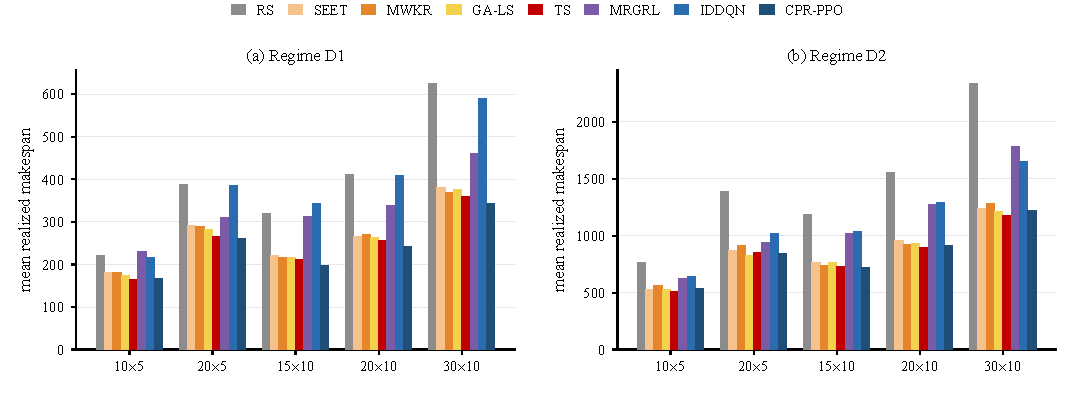
\includegraphics[width=0.84\textwidth]{figs/figS1_makespan.pdf}
\caption{Mean realized makespan per unit, with both regimes on a shared axis.}
\label{fig:S-makespan}
\end{figure*}

\begin{table*}[!t]
\caption{Per-unit rank of every method and gap difference of CPR-PPO against TS in percentage points; negative values favour CPR-PPO.}
\label{tab:S-ranks}
\centering
\scriptsize
\setlength{\tabcolsep}{6pt}
\begin{tabular}{@{}llccccccccr@{}}
\toprule
Regime & Size & RS & SEET & MWKR & GA-LS & TS & MRGRL & IDDQN & CPR-PPO & $\Delta$ vs TS\\
\midrule
D1 & $10\times5$ & 7.0 & 5.0 & 4.0 & 3.0 & \textbf{1.0} & 8.0 & \cellcolor{bestblue}6.0 & 2.0 & +0.80\\
D1 & $20\times5$ & 8.0 & 5.0 & 4.0 & 3.0 & 2.0 & 6.0 & \cellcolor{bestblue}7.0 & 1.0 & -2.02\\
D1 & $15\times10$ & 7.0 & 5.0 & 3.0 & 4.0 & 2.0 & 6.0 & \cellcolor{bestblue}8.0 & 1.0 & -7.46\\
D1 & $20\times10$ & 8.0 & 4.0 & 5.0 & 3.0 & 2.0 & 6.0 & \cellcolor{bestblue}7.0 & 1.0 & -6.03\\
D1 & $30\times10$ & 8.0 & 5.0 & 3.0 & 4.0 & 2.0 & 6.0 & \cellcolor{bestblue}7.0 & 1.0 & -4.81\\
D2 & $10\times5$ & 8.0 & 3.0 & 5.0 & 2.0 & \textbf{1.0} & 6.0 & \cellcolor{bestblue}7.0 & 4.0 & +5.20\\
D2 & $20\times5$ & 8.0 & 4.0 & 5.0 & \textbf{1.0} & 3.0 & 6.0 & \cellcolor{bestblue}7.0 & 2.0 & -1.80\\
D2 & $15\times10$ & 8.0 & 4.0 & 3.0 & 5.0 & 2.0 & 6.0 & \cellcolor{bestblue}7.0 & 1.0 & -1.49\\
D2 & $20\times10$ & 8.0 & 5.0 & 3.0 & 4.0 & \textbf{1.0} & 6.0 & \cellcolor{bestblue}7.0 & 2.0 & +1.64\\
D2 & $30\times10$ & 8.0 & 4.0 & 5.0 & 2.0 & \textbf{1.0} & 7.0 & \cellcolor{bestblue}6.0 & 3.0 & +3.42\\
\midrule
Mean & -- & 7.80 & 4.40 & 4.00 & 3.10 & 1.70 & 6.30 & 6.90 & 1.80 & -1.25\\
\bottomrule
\end{tabular}
\end{table*}


Fig.~\ref{fig:S-transfer} expresses the same information in two ways: the improvement over right shifting as a function of size under D1, and the mean rank over the ten units. The improvement curve of CPR-PPO is the flattest among the learned methods, which is the property that a recovery policy has to preserve when the shop grows.

\begin{figure*}[!t]
\centering
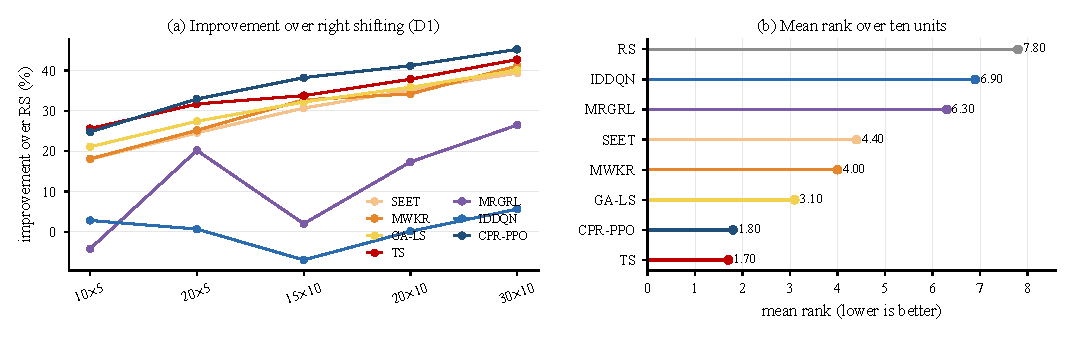
\includegraphics[width=0.70\textwidth]{figs/figS2_transfer.pdf}
\caption{Improvement over right shifting under D1, and mean rank over the ten units.}
\label{fig:S-transfer}
\end{figure*}

\subsection{Recovery Trajectory and Gap Structure}
\label{sec:S-structure}

Fig.~\ref{fig:S-gantt} plots one complete trajectory of CPR-PPO on a $20\times10$ instance of D1 with failure stream 79000000. Each colour identifies one job, hatched bars are corrective repairs, pale bars are processing lost when an interrupted operation restarts, and the lower rail marks the intervals in which each machine is under repair. The instance contains twenty-one breakdowns, the repair occupancy of individual machines ranges from 0\% to 37\% of the horizon, and 122.3 machine-time units of processing are lost to restarted operations.

\begin{figure*}[!t]
\centering
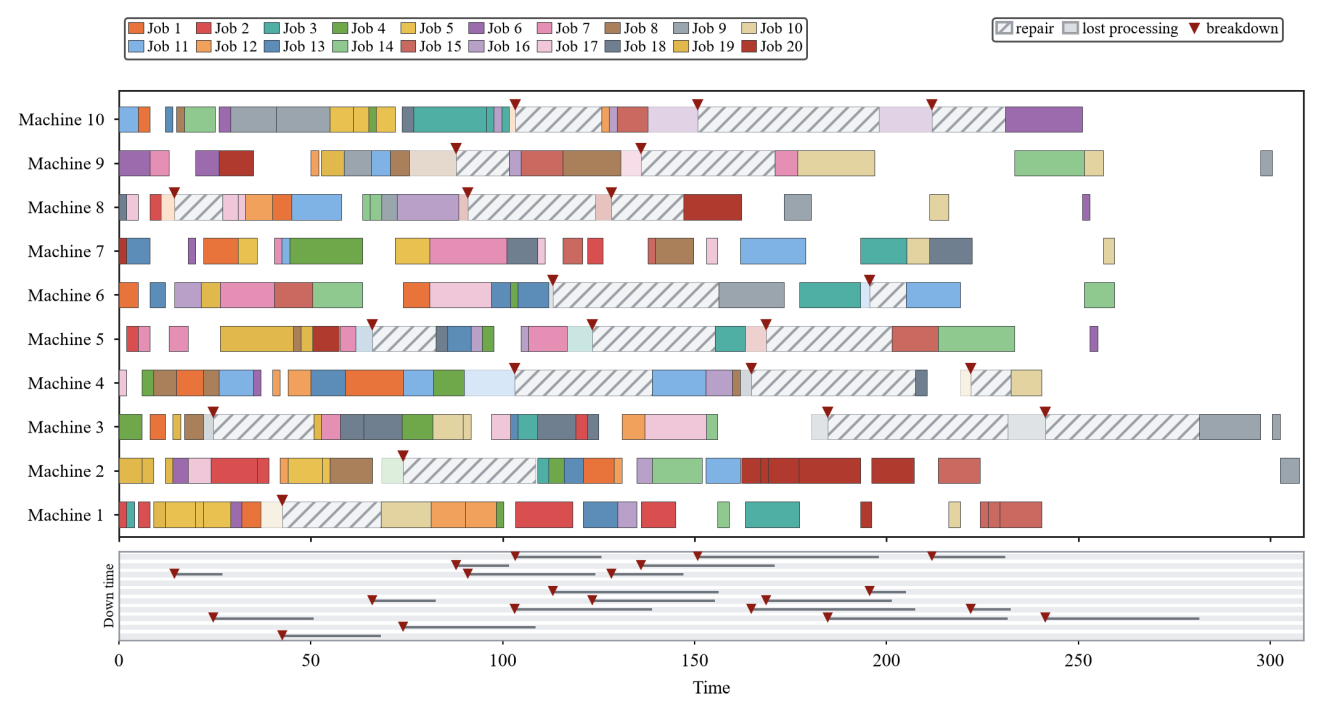
\includegraphics[width=0.80\textwidth]{figs/gantt.png}
\caption{Recovery schedule of CPR-PPO on a $20\times10$ instance under D1 ($\hat{C}_{\max}=307.50$). Hatched bars are repairs, pale bars lost processing, triangles breakdowns, and the lower rail repair intervals.}
\label{fig:S-gantt}
\end{figure*}

Fig.~\ref{fig:S-gapmap} displays the relative excess of every method over the best method of each unit, with the absolute makespan annotated in each cell. The figure makes the two failure modes of the baselines explicit: the rule-based methods degrade smoothly with size, whereas the adapted DRL baselines degrade abruptly on the largest D2 unit, where the excess of IDDQN reaches 43.0\%.

\begin{figure*}[!t]
\centering
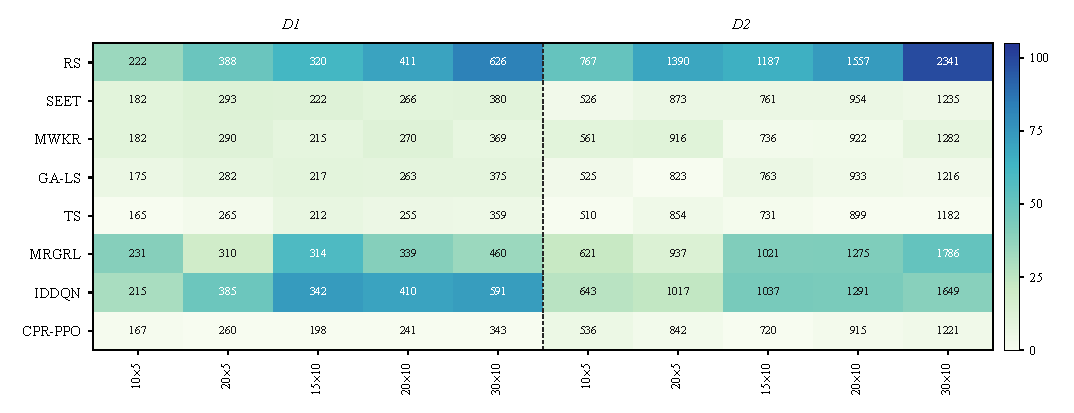
\includegraphics[width=0.78\textwidth]{figs/figS4_makespan_map.pdf}
\caption{Mean realized makespan (annotation) and excess over the best method per unit (colour).}
\label{fig:S-gapmap}
\end{figure*}

\section{Reproducibility Protocol}
\label{sec:S-repro}

\subsection{Software and Seeds}
\label{sec:S-software}

All experiments run on Python 3.12 with CPU PyTorch 2.7.0 and a NumPy implementation of the shop simulator. One training seed is retained per unit, three failure streams and three search seeds are replayed per instance, and the instance is the unit of paired comparison.

\end{document}
